%!TEX root = ../docu.tex
\section{Einleitung}
\subsection{Motivation}
Mobile Endgeräte wie Tablets und Smartphones nehmen stetig einen höhere Bedeutung im Alltag vieler Menschen ein. Dies bestätigen aktuelle Verkaufszahlen von erwähnten Geräten. Diese sind in Abbildung \ref{sale1}\footnote{http://www.statista.com/statistics/74592/quarterly-worldwide-smartphone-sales-by-operating-system-since-2009/} ersichtlich. Sie bestimmten die Art und weise der Informationsverarbeitung und beschafft sowie die Kommunikation derer die diese Geräte benutzen.


\begin{figure}
\begin{center}
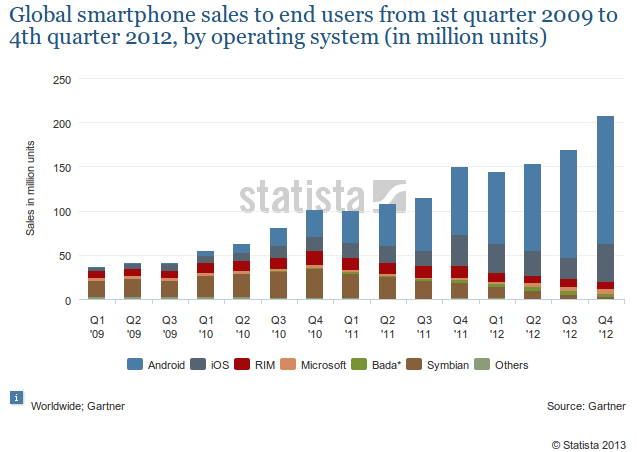
\includegraphics[scale=0.6]{images/sale}
\caption{Verkaufszahlen von Smartphones weltweit nach Plattform}
\label{sale1}
\end{center}
\end{figure}


Aktueller Vorreiter der Brache ist das auf Linux basierende Betriebssystem Android von Google Inc. . Die wachsende Beliebtheit dieses Betriebssystems für Tablets und Smartphone macht es umso interessanter für Entwickler Applikationen und Services für Geräte zu entwickeln die dieses Betriebssystem nutzen.

Um einen Einblick in die Entwicklung von Applikationen für das mobile Betriebssystem haben wir uns daher für die Entwicklung einer Applikation für die besagte Plattform entschieden.

Die geplante Applikation soll einen vorbestimmten Zweck dienen und einen nutzen erfüllen.

\subsection{Vorwort}
Die Arbeit soll Einblicke in die Entwicklung von Applikationen für das Betriebssystem Android gewähren. Es werden die Grundstrukturen vorgestellt und erläutert. Diese Grundstrukturen sind äußerst wichtig um die Art und Weise wie Applikationen auf der Plattform ausgeführt werden und vom Nutzer verwendet werden.

Abschließend werden verschiedene Probleme und Lösungswege wären den konzeptionieren und Implementierung sowie der Projektbearbeitung erläutert.

Dies beinhaltet verschiedene projektorganisatorische Elemente wie Versionierung und Projektplanung (\ref{proj}). die Kapitel beschäftigen sich mit verschiebenden Herangehensweisen für die Projektarbeit in kleinen Teams sowie die Funktionsweise und Anwendung.

Des weiteren werden verschiedene Schritte von Kozeptionierung sowie Implementierung verschiedener Komponentenstrukturen der Applikation diskutiert und ausgewertet. Das letztendliche Ziel der Arbeit ist eine nutzbare zweckgerichtete Applikation.

Diese Applikation soll dazu dienen die Grundlagen der Android Plattform zu erlangen. Dies beinhaltet die Funktionsweise von nativen Android Applikationen (\ref{natand}) sowie der Android SDK. Ein tiefes Verständnis für die eigentliche Android Betriebssystem erleichtert die Entwicklung und das Verständnis über verschiedene betriebssystemspezifischen Eigenheiten. Diese und weiter Grundlagen sollen ebenso in dieser Arbeit behandelt und diskutiert werden.
